\begin{center}
	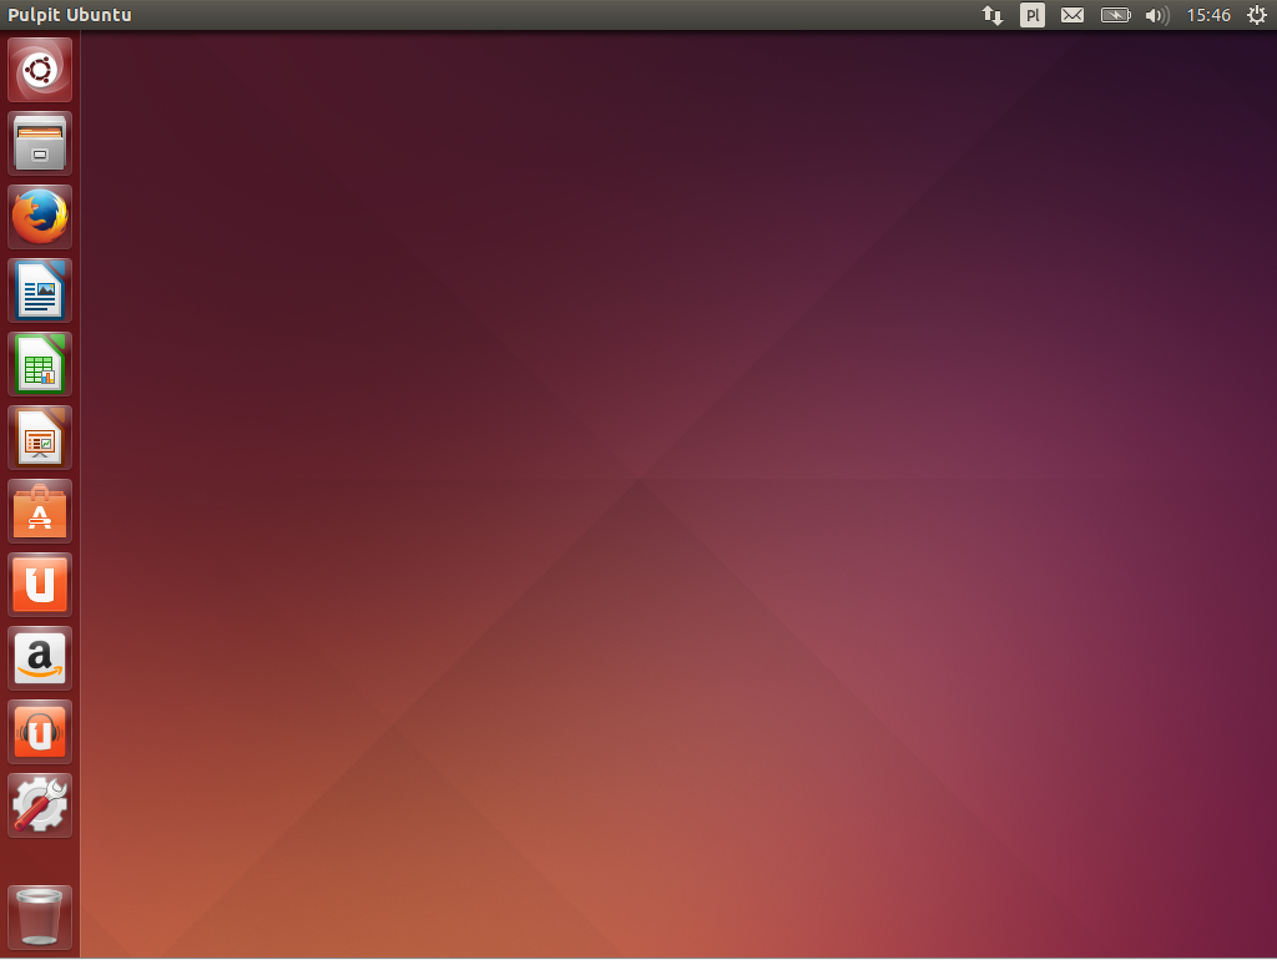
\includegraphics[width=\linewidth]{images/unity_desktop.png}
\end{center}

Po zalogowaniu się do systemu Twoim oczom ukaże się Pulpit. Widać na nim trzy elementy: przestrzeń roboczą wypełniającą większą część ekranu oraz dwa panele. Panel poziomy, zwany \textcolor{ubuntu_orange}{Panelem Menu}, umieszczony na górze ekranu. Panel pionowy to \textcolor{ubuntu_orange}{Launcher} lub inaczej Panel Uruchamiania, zlokalizowany jest po lewej stronie ekranu.

\subsubsection{Zmiana tła pulpitu}
Aby zmienić tło pulpitu (inaczej: tapetę) kliknij \textbf{prawym przyciskiem myszy} na wolnej przestrzeni roboczej i z menu kontekstowego wybierz \textcolor{ubuntu_orange}{Zmień tło pulpitu}

\begin{wrapfigure}{r}{0.5\textwidth}
	\vspace{-10pt}
	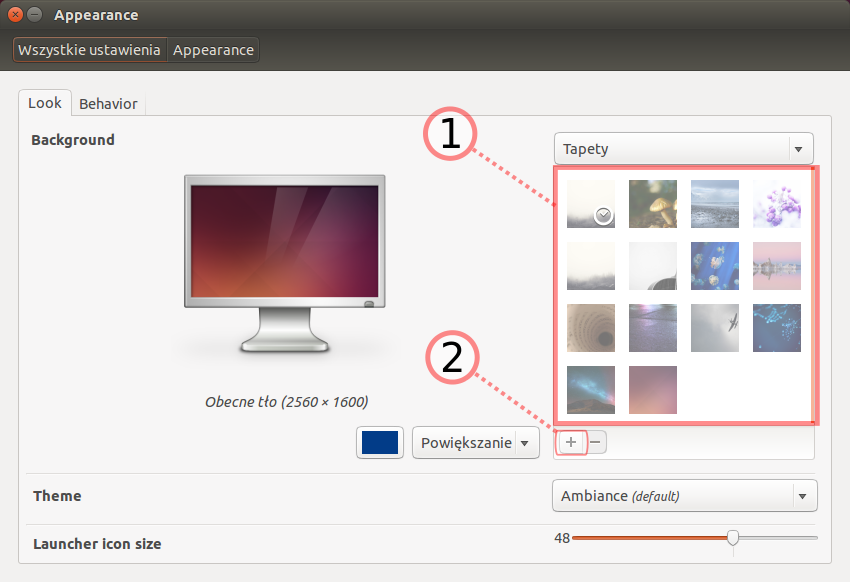
\includegraphics[width=\linewidth]{images/unity_zmiana_tapety.png}
\end{wrapfigure}

Z listy zaznaczonej jako \textcolor{ubuntu_orange}{(}1\textcolor{ubuntu_orange}{)} możesz wybrać jedną z gotowych tapet. Kliknij na przycisk plus \textcolor{ubuntu_orange}{(}2\textcolor{ubuntu_orange}{)} aby otworzyć menadźer plików i wskazać inny plik graficzny na dysku twardym. Plik ten zostanie użyty jako tapeta.

W tym oknie możesz też dokonać pewnych modyfikacji środowiska graficznego Unity. Zachęcamy do eksperymentów. Wszelkie zmiany są wprowadzane na żywo.